\documentclass[10pt]{article}
\usepackage[utf8]{inputenc}
\usepackage[doublespacing]{setspace}
\usepackage{textcomp}
\usepackage{amsmath,amssymb,amsthm}
\usepackage{fancyhdr}
\usepackage{lastpage}
\usepackage[]{hyperref}
\usepackage[pdftex]{graphicx}
\usepackage{ctex}
\usepackage{booktabs}
\usepackage{subfigure}
\usepackage{titlesec}
\usepackage{listings}
\usepackage{enumerate}
\usepackage{bm}
\usepackage{float}
\usepackage{url}
\usepackage[english]{babel}
%\allowdisplaybreaks
\renewcommand{\contentsname}{\centerline{Contents}}
\pagestyle{fancy}
\author{D}
\def\name{D}
\lhead{Big Data}
\chead{}
\rhead{\name}
\cfoot{-\space\thepage\space-}
\newtheorem{exer}{\bm{$Exercise$}}
\newtheorem{prob}{\bm{$Problem$}}
\newtheorem{bonus}{\bm{$Bonus\;Problem$}}
\newcommand{\tabincell}[2]{\begin{tabular}{@{}#1@{}}#2\end{tabular}}
\CTEXoptions[today=old]

\begin{document}

\title{Assignment One}
\date{\today}
\maketitle
\thispagestyle{fancy}
\thispagestyle{fancy}

\begin{prob}
\end{prob}
\begin{enumerate}[1)]
\vspace{3mm}

\item
The observations for a response random variable $\pmb{y}$ are written as a vector, where
\begin{align*}
\pmb{y}=
  \begin{bmatrix}
    5\\
    9\\
    13
  \end{bmatrix}
,
\end{align*}
and the observations for the explanatory variable $\pmb{X}$ are written as a matrix, where
\begin{align*}
\pmb{X}=
  \begin{bmatrix}
    1 & 3\\
    1 & 4\\
    1 & 5
  \end{bmatrix}
.
\end{align*}
Referring to page 51 of the simple linear regression lecture notes\footnote{Reale, M. (2020). \textit{Lecture notes in big data}. Unpublished manuscript.}, straightforwardly, we get the ordinary least squares estimates of the coefficients, which are written as a matrix $\pmb{\hat{\beta}}$, where
\begin{align*}
\pmb{\hat{\beta}}&=(\pmb{X\textsuperscript{$\prime$}}\pmb{X})^{-1}\pmb{X\textsuperscript{$\prime$}}\pmb{y}.
\end{align*}
Based on the lecture notes, by hand we have two approaches to acquire $\pmb{\hat{\beta}}$.\\
The first approach is direct matrix calculation.\\
\begin{align*}
\pmb{\hat{\beta}}&=(\pmb{X\textsuperscript{$\prime$}}\pmb{X})^{-1}\pmb{X\textsuperscript{$\prime$}}\pmb{y}\\
&=(
  \begin{bmatrix}
    1 & 3\\
    1 & 4\\
    1 & 5
  \end{bmatrix}
'
  \begin{bmatrix}
    1 & 3\\
    1 & 4\\
    1 & 5
  \end{bmatrix}
)^{-1}
  \begin{bmatrix}
    1 & 3\\
    1 & 4\\
    1 & 5
  \end{bmatrix}
'
  \begin{bmatrix}
    5\\
    9\\
    13
  \end{bmatrix}
\\
&=
  \begin{bmatrix}
    3 & 12\\
    12 & 50
  \end{bmatrix}
^{-1}
  \begin{bmatrix}
    1 & 3\\
    1 & 4\\
    1 & 5
  \end{bmatrix}
'
  \begin{bmatrix}
    5\\
    9\\
    13
  \end{bmatrix}
\\
&=
  \begin{bmatrix}
    \frac{25}{3} & -2\\
    -2 & \frac{1}{2}
  \end{bmatrix}
  \begin{bmatrix}
    1 & 3\\
    1 & 4\\
    1 & 5
  \end{bmatrix}
'
  \begin{bmatrix}
    5\\
    9\\
    13
  \end{bmatrix}
\\
&=
  \begin{bmatrix}
    \frac{7}{3} & \frac{1}{3} & -\frac{5}{3}\\
    -\frac{1}{2} & 0 & \frac{1}{2}\\
  \end{bmatrix}
  \begin{bmatrix}
    5\\
    9\\
    13
  \end{bmatrix}
\\
&=
  \begin{bmatrix}
    -7\\
    4
  \end{bmatrix}
.
\end{align*}
The second approach is using the formulas on page 51.\\
Since $(\pmb{X\textsuperscript{$\prime$}}\pmb{X})^{-1}=\frac{1}{n\sum(x_i-\bar{x})^2}
  \begin{bmatrix}
    \sum{x_i^2} & -\sum{x_i}\\
    -\sum{x_i} & n
  \end{bmatrix}
$
and $\pmb{X\textsuperscript{$\prime$}}\pmb{y}=
  \begin{bmatrix}
    \sum{y_i}\\
    \sum{x_i y_i}
  \end{bmatrix}
$, we have
\begin{align*}
\pmb{\hat{\beta}}=\frac{1}{n\sum(x_i-\bar{x})^2}
  \begin{bmatrix}
    \sum{x_i^2} & -\sum{x_i}\\
    -\sum{x_i} & n
  \end{bmatrix}
  \begin{bmatrix}
    \sum{y_i}\\
    \sum{x_i y_i}
  \end{bmatrix}
.
\end{align*}
Using the given matrices, we get $n=3$, $\bar{x}=4$, $\sum(x_i-\bar{x})^2=2$, $\sum{x^2_i}=50$, $-\sum{x_i}=-12$, $\sum{y_i}=27$ and $\sum{x_i y_i}=116$. Therefore,
\begin{align*}
\pmb{\hat{\beta}}&=\frac{1}{3\times2}
  \begin{bmatrix}
    50 & -12\\
    -12 & 3
  \end{bmatrix}
  \begin{bmatrix}
    27\\
    116
  \end{bmatrix}
\\
&=\frac{1}{6}
  \begin{bmatrix}
    50\times27-12\times116\\
    -12\times27+3\times116
  \end{bmatrix}
\\
&=\frac{1}{6}
  \begin{bmatrix}
    -42\\
    24
  \end{bmatrix}
\\
&=
  \begin{bmatrix}
    -7\\
    4
  \end{bmatrix}
\end{align*}
The two approaches reach the same result. Hence, we get the required coefficients $\hat{\beta}_0=-7$ and $\hat{\beta}_1=4$.

\item
Referring to page 53, we get the estimated residuals $\pmb{\hat{\epsilon}}$, where
\begin{align*}
\pmb{\hat{\epsilon}}&=\pmb{y}-\pmb{X\hat{\beta}}\\
&=
  \begin{bmatrix}
    5\\
    9\\
    13
  \end{bmatrix}
-
  \begin{bmatrix}
    -7+4\times3\\
    -7+4\times4\\
    -7+4\times5
  \end{bmatrix}
\\
&=
  \begin{bmatrix}
    5\\
    9\\
    13
  \end{bmatrix}
-
  \begin{bmatrix}
    5\\
    9\\
    13
  \end{bmatrix}
\\
&=
  \begin{bmatrix}
    0\\
    0\\
    0
  \end{bmatrix}
\end{align*}
Hence, the estimates of the residuals $\pmb{\hat{\epsilon}}$ are $
  \begin{bmatrix}
    0 & 0 & 0
  \end{bmatrix}\textsuperscript{$\prime$}$.

\item
Please see ``032620RA.Rmd''.

\item
Please see ``032620RA.Rmd''.

\end{enumerate}
\vspace{3mm}

\begin{prob}
\end{prob}
\begin{enumerate}[1)]
\vspace{3mm}

\item
Given $\pmb{X}$, where
\begin{align*}
\pmb{X}=
  \begin{bmatrix}
    1 & 2\\
    1 & 2\\
    1 & 2
  \end{bmatrix}
,
\end{align*}
and $\pmb{y}$ unchanged, we repeat all the approaches in the previous problem.\\
First, using matrix calculation by hand,
\begin{align*}
\pmb{\hat{\beta}}&=(\pmb{X\textsuperscript{$\prime$}}\pmb{X})^{-1}\pmb{X\textsuperscript{$\prime$}}\pmb{y}\\
&=(
  \begin{bmatrix}
    1 & 2\\
    1 & 2\\
    1 & 2
  \end{bmatrix}
'
  \begin{bmatrix}
    1 & 2\\
    1 & 2\\
    1 & 2
  \end{bmatrix}
)^{-1}
  \begin{bmatrix}
    1 & 2\\
    1 & 2\\
    1 & 2
  \end{bmatrix}
'
  \begin{bmatrix}
    5\\
    9\\
    13
  \end{bmatrix}
\\
&=
  \begin{bmatrix}
    3 & 6\\
    6 & 12
  \end{bmatrix}
^{-1}
  \begin{bmatrix}
    1 & 2\\
    1 & 2\\
    1 & 2
  \end{bmatrix}
'
  \begin{bmatrix}
    5\\
    9\\
    13
  \end{bmatrix}
.
\end{align*}
Since $
  \begin{vmatrix}
    3 & 6\\
    6 & 12
  \end{vmatrix}
=0$,$
  \begin{bmatrix}
    3 & 6\\
    6 & 12
  \end{bmatrix}
$ is not invertible. We can not proceed the calculation and thus can not acquire $\pmb{\hat{\beta}}$.\\
Second, using the formulas in the lecture notes, where $\pmb{\hat{\beta}}=(\pmb{X\textsuperscript{$\prime$}}\pmb{X})^{-1}\pmb{X\textsuperscript{$\prime$}}\pmb{y}=\frac{1}{n\sum(x_i-\bar{x})^2}
  \begin{bmatrix}
    \sum{x_i^2} & -\sum{x_i}\\
    -\sum{x_i} & n
  \end{bmatrix}
  \begin{bmatrix}
    \sum{y_i}\\
    \sum{x_i y_i}
  \end{bmatrix}$, since $\frac{1}{n\sum(x_i-\bar{x})^2}=\frac{1}{3\sum(0)^2}=\frac{1}{0}$ is undefined, we can not acquire $\pmb{\hat{\beta}}$.\\
Third, using matrix calculation in R, we get an non-conformable arguments error.\\
Fourth, using the function \textbf{lm} in R, we get the following outputs,\\
\begin{table}[H]
\centering
\begin{tabular}{rr}
\multicolumn{2}{l}{Coefficients:} \\
(Intercept)          & X          \\
9                    & NA
\end{tabular}
\end{table}
showing $\hat{\beta}_0=9$ and $\hat{\beta}_1$ is not applicable.\\
In all, the complete coefficient estimate matrix can not be acquired.

\item
A statistical explanation.\\
We recall the matrix calculation, where
\begin{align*}
\pmb{\hat{\beta}}&=(\pmb{X\textsuperscript{$\prime$}}\pmb{X})^{-1}\pmb{X\textsuperscript{$\prime$}}\pmb{y}\\
&=(
  \begin{bmatrix}
    1 & 2\\
    1 & 2\\
    1 & 2
  \end{bmatrix}
'
  \begin{bmatrix}
    1 & 2\\
    1 & 2\\
    1 & 2
  \end{bmatrix}
)^{-1}
  \begin{bmatrix}
    1 & 2\\
    1 & 2\\
    1 & 2
  \end{bmatrix}
'
  \begin{bmatrix}
    5\\
    9\\
    13
  \end{bmatrix}
\\
&=
  \begin{bmatrix}
    3 & 6\\
    6 & 12
  \end{bmatrix}
^{-1}
  \begin{bmatrix}
    1 & 2\\
    1 & 2\\
    1 & 2
  \end{bmatrix}
'
  \begin{bmatrix}
    5\\
    9\\
    13
  \end{bmatrix}
.
\end{align*}
Since the determinant of $
  \begin{bmatrix}
    3 & 6\\
    6 & 12
  \end{bmatrix}
$ is $
  \begin{vmatrix}
    3 & 6\\
    6 & 12
  \end{vmatrix}
$, where $
  \begin{vmatrix}
    3 & 6\\
    6 & 12
  \end{vmatrix}
=0$,
$
  \begin{bmatrix}
    3 & 6\\
    6 & 12
  \end{bmatrix}
$ is singular (not full rank) and thus not invertible. Hence, $\pmb{\hat{\beta}}$ can not be acquired.\\
A geometric explanation.\\
\begin{figure}[H]
  \centering
  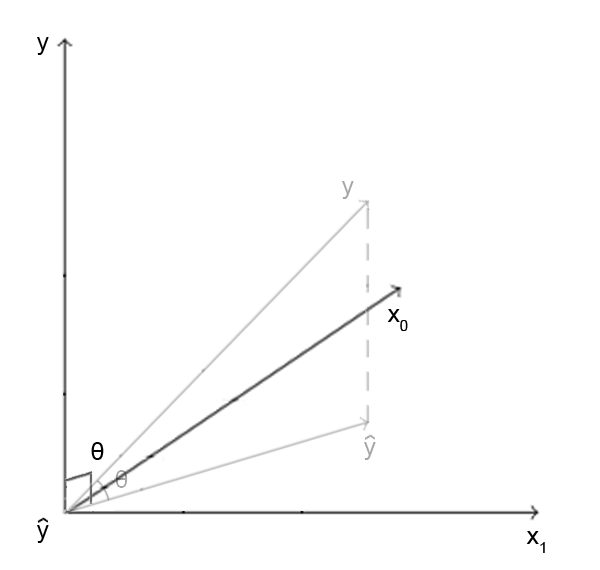
\includegraphics[scale=0.5]{p22a.png}
  \caption{Geometry of OLS}
\end{figure}
Let $\pmb{H}$ be a hat matrix, where $\pmb{\hat{y}}=\pmb{H}\pmb{y}$, so we have
\begin{align*}
\pmb{H}\pmb{y}=\hat{\beta}_0\pmb{x_0}+\hat{\beta}_1\pmb{x_1}.
\end{align*}
Geometrically, $\pmb{\hat{y}}$ is the orthogonal projection of $\pmb{y}$; $cos(\theta)$ implies the correlation between $\pmb{y}$ and $\pmb{X}$.\\
In this case where $cos(\theta)=0$, $\pmb{y}$ is perpendicular to the $x_0x_1$ plane, the projection $\pmb{\hat{y}}$ is $\pmb{0}$ and the correlation is zero, i.e. unexplainability.\\
Use the graph. Lines in gray show the general form (full rank); lines in black are for this case (not full rank).
\end{enumerate}

\end{document}

% Comment: 2b) This is a case of collinearity between the intercept and the explanatory variable. Both intercept and variable provide the same information, hence one of them is redundant. The vector of the intercept and the vector of X observations have identical directions, although with different length. Hence the area of the parallelogram defined by the two vectors is zero.
